\documentclass{article}
\usepackage{pgfplots}

\pgfplotsset{compat=1.3}
\usepgfplotslibrary{patchplots}

\begin{document}
\thispagestyle{empty}

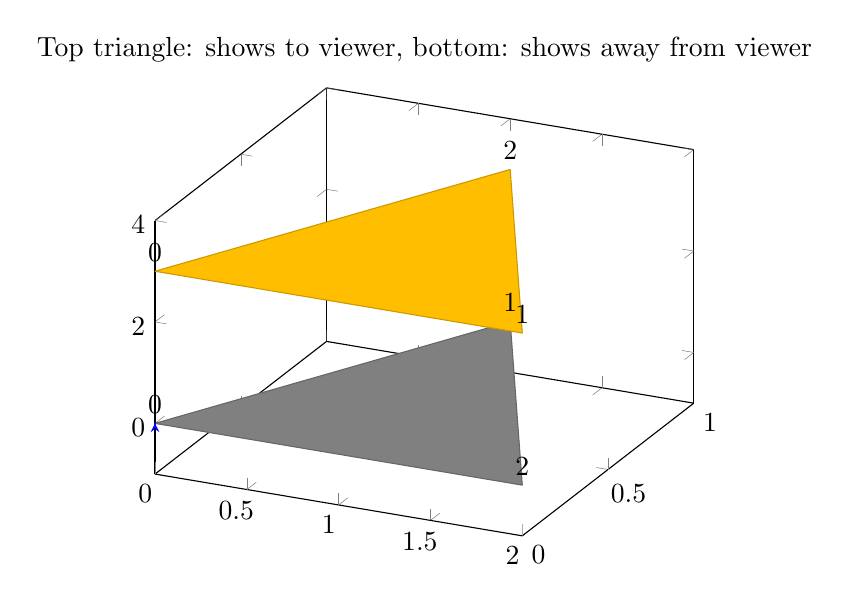
\begin{tikzpicture}
%\tracingmacros=2 \tracingcommands=2
    \begin{axis}[
	zmin=-1,zmax=4,
	title={Top triangle: shows to viewer, bottom: shows away from viewer},
		nodes near coords,point meta=explicit,
		colormap/blackwhite,
		mesh/interior colormap name={hot},
		clip=false,
	]
    \addplot3[patch,table/meta=m]
    table {
        x y z m
        0 0 0 0
        1 1 0 1
        2 0 0 2
% empty lines do not hurt, they are ignored here:

        0 0 3 0
        2 0 3 1
        1 1 3 2
    };
	\draw[-stealth,blue] (axis cs:0,0,0)  \pgfextra{\pgfpathlineto{\pgfpointadd{\pgfplotspointaxisxyz000}{\pgfplotspointviewdir}}};
    \end{axis}
\end{tikzpicture}

\message{mit patch to triangles:^^J}%
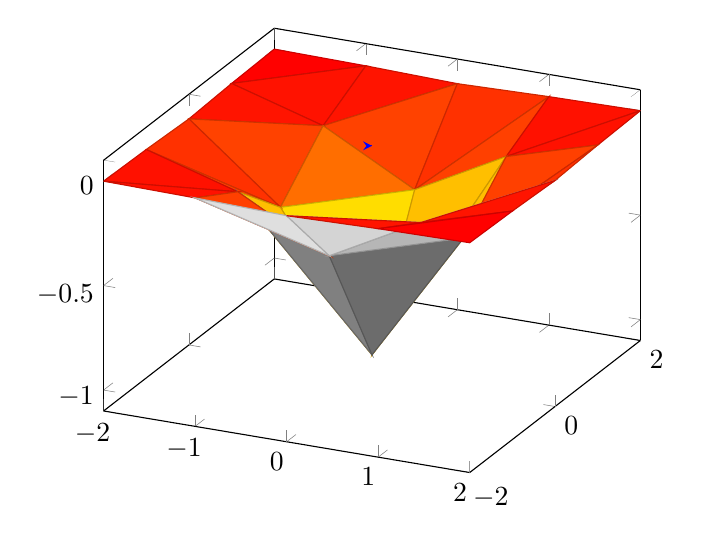
\begin{tikzpicture}
%\tracingmacros=2 \tracingcommands=2
	\begin{axis}[domain=-2:2,
		mesh/interior colormap name={hot},
		colormap/blackwhite,
		samples=5,
		%nodes near coords=\coordindex,
		patch to triangles,
		%mesh/show normals,
	]
	\addplot3[surf] {-exp(-x^2-y^2)};
	\draw[-stealth,blue] (axis cs:0,0,0)  \pgfextra{\pgfpathlineto{\pgfpointadd{\pgfplotspointaxisxyz000}{\pgfplotspointviewdir}}};
	\end{axis}
\end{tikzpicture}

\message{ohne patch to triangles:^^J}%
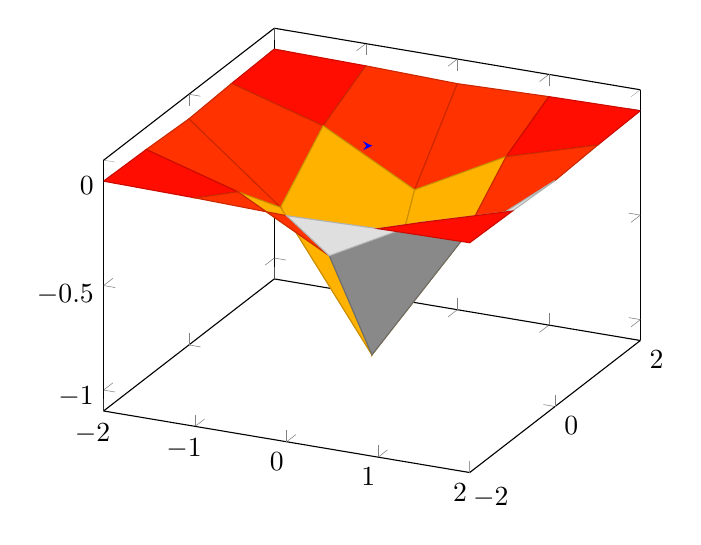
\begin{tikzpicture}
%\tracingmacros=2 \tracingcommands=2
	\begin{axis}[domain=-2:2,
		mesh/interior colormap name={hot},
		colormap/blackwhite,
		samples=5,
		%disabledatascaling,
		%nodes near coords=\coordindex,
		%patch to triangles,
		%mesh/show normals,
	]
	\addplot3[surf] {-exp(-x^2-y^2)};
	\draw[-stealth,blue] (axis cs:0,0,0)  \pgfextra{\pgfpathlineto{\pgfpointadd{\pgfplotspointaxisxyz000}{\pgfplotspointviewdir}}};
	\end{axis}
\end{tikzpicture}


\message{fancy cone:^^J}%
%\end{document}
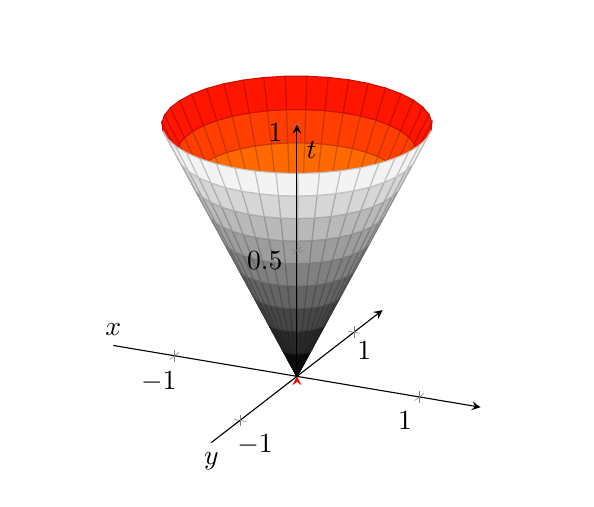
\begin{tikzpicture}
%\tracingmacros=2 \tracingcommands=2
\begin{axis}[
  axis lines=center,
  axis on top,
  xlabel={$x$}, ylabel={$y$}, zlabel={$t$},
  domain=0:1,
  y domain=0:2*pi,
  xmin=-1.5, xmax=1.5,
  ymin=-1.5, ymax=1.5, zmin=0.0,
 		every axis x label/.style={at={(rel axis cs:0,0.5,0)},anchor=south},
		every axis y label/.style={at={(rel axis cs:0.5,0,0)},anchor=north},
		every axis z label/.style={at={(rel axis cs:0.5,0.5,0.9)},anchor=west},
		mesh/interior colormap name=hot,
		mesh/interior colormap thresh=0,
		colormap/blackwhite, 
		%disabledatascaling,
		%patch to triangles,
		%mesh/show normals,
 	 samples=10,
	 samples y=40,
	 z buffer=sort,
 ]
%  \scope
%  \addplot3 [/tikz/clip,red,samples=30,domain=0:2*pi,samples y=1] ({cos(deg(x))},{sin(deg(x))},{1});
  \addplot3 [surf, shader=faceted] ({x*cos(deg(y))},{x*sin(deg(y))},{x});
%  \endscope

	\draw[-stealth,red] (axis cs:0,0,0)  \pgfextra{\pgfpathlineto{\pgfpointadd{\pgfplotspointaxisxyz000}{\pgfplotspointviewdir}}};
\end{axis}
\end{tikzpicture}

\end{document}

